% THIS IS SIGPROC-SP.TEX - VERSION 3.1
% WORKS WITH V3.2SP OF ACM_PROC_ARTICLE-SP.CLS
% APRIL 2009
%
% It is an example file showing how to use the 'acm_proc_article-sp.cls' V3.2SP
% LaTeX2e document class file for Conference Proceedings submissions.
% ----------------------------------------------------------------------------------------------------------------
% This .tex file (and associated .cls V3.2SP) *DOES NOT* produce:
%       1) The Permission Statement
%       2) The Conference (location) Info information
%       3) The Copyright Line with ACM data
%       4) Page numbering
% ---------------------------------------------------------------------------------------------------------------
% It is an example which *does* use the .bib file (from which the .bbl file
% is produced).
% REMEMBER HOWEVER: After having produced the .bbl file,
% and prior to final submission,
% you need to 'insert'  your .bbl file into your source .tex file so as to provide
% ONE 'self-contained' source file.
%
% Questions regarding SIGS should be sent to
% Adrienne Griscti ---> griscti@acm.org
%
% Questions/suggestions regarding the guidelines, .tex and .cls files, etc. to
% Gerald Murray ---> murray@hq.acm.org
%
% For tracking purposes - this is V3.1SP - APRIL 2009

\documentclass{acm_proc_article-sp}
\usepackage[numbers, sort, compress]{natbib}
\usepackage{graphics}
\usepackage{graphicx}
\usepackage{epstopdf}
\usepackage{color}
\usepackage{hyperref}
\usepackage{pdfsync}
\usepackage{mdwlist}

\begin{document}

%\title{A Sample {\ttlit ACM} SIG Proceedings Paper in LaTeX
%Format\titlenote{(Does NOT produce the permission block, copyright information nor page numbering). For use with ACM\_PROC\_ARTICLE-SP.CLS. Supported by ACM.}}

\newif\ifdraft
\drafttrue                                                                                                   

\ifdraft
 \newcommand{\rananote}[1]{ {\textcolor{blue}    { ***Omer:     #1 }}}
 \newcommand{\jkimnote}[1]{{\textcolor{green}   { ***Joohyun:   #1 }}}
 \newcommand{\jhanote}[1]{  {\textcolor{red}     { ***SJ: #1 }}}
  \newcommand{\smnote}[1]{  {\textcolor{blue}     { ***sharath: #1 }}}
 \newcommand{\todo}[1]{  {\textcolor{red}     { ***TODO: #1 }}}
 \newcommand{\fix}[1]{  {\textcolor{red}     { ***FIX: #1 }}}

\else
 \newcommand{\rananote}[1]{}
 \newcommand{\jkimnote}[1]{}
 \newcommand{\jhanote}[1]{}
 \newcommand{\todo}[1]{  {\textcolor{red}     { ***TODO: #1 }}}
 \newcommand{\fix}[1]{}                                                                                     
\fi

\title{Characterizing Deep Sequencing Analytics Using BFAST: Towards a
  Scalable Distributed Architecture for Next-Generation Sequencing
  Data}

% \title{Exploring the RNA Folding Energy Landscape with
%   Boltzmann-Weighted Sampling of Secondary Structures: Enhancing the
%   Biological Discovery with Adaptive Distributed Application
%   Management System (ADAMS) }

%\subtitle{[Extended Abstract]
%\titlenote{A full version of this paper is available as
%\textit{Author's Guide to Preparing ACM SIG Proceedings Using
%\LaTeX$2_\epsilon$\ and BibTeX} at
%\texttt{www.acm.org/eaddress.htm}}}
%
% You need the command \numberofauthors to handle the 'placement
% and alignment' of the authors beneath the title.
%
% For aesthetic reasons, we recommend 'three authors at a time'
% i.e. three 'name/affiliation blocks' be placed beneath the title.
%
% NOTE: You are NOT restricted in how many 'rows' of
% "name/affiliations" may appear. We just ask that you restrict
% the number of 'columns' to three.
%
% Because of the available 'opening page real-estate'
% we ask you to refrain from putting more than six authors
% (two rows with three columns) beneath the article title.
% More than six makes the first-page appear very cluttered indeed.
%
% Use the \alignauthor commands to handle the names
% and affiliations for an 'aesthetic maximum' of six authors.
% Add names, affiliations, addresses for
% the seventh etc. author(s) as the argument for the
% \additionalauthors command.
% These 'additional authors' will be output/set for you
% without further effort on your part as the last section in
% the body of your article BEFORE References or any Appendices.

\numberofauthors{6} %  in this sample file, there are a *total*
% of EIGHT authors. SIX appear on the 'first-page' (for formatting
% reasons) and the remaining two appear in the \additionalauthors section.
%
\author{
% You can go ahead and credit any number of authors here,
% e.g. one 'row of three' or two rows (consisting of one row of three
% and a second row of one, two or three).
%
% The command \alignauthor (no curly braces needed) should
% precede each author name, affiliation/snail-mail address and
% e-mail address. Additionally, tag each line of
% affiliation/address with \affaddr, and tag the
% e-mail address with \email.
%
\alignauthor Joohyun Kim\\
       \affaddr{Center for Computation and Technology}\\
       \affaddr{Louisiana State University}\\
       \affaddr{216 Johnston}\\
       \affaddr{Baton Rouge, LA} \\
       \email{jhkim@cct.lsu.edu}
\alignauthor Sharath Maddineni\\
       \affaddr{Center for Computation and Technology}\\
       \affaddr{Louisiana State University}\\
       \affaddr{216 Johnston}\\
       \affaddr{Baton Rouge, LA}
\alignauthor Shantenu Jha\titlenote{Author for correspondence}\\
      \affaddr{Center for Computation and Technology}\\
     \affaddr{Louisiana State Unvierstiy}\\
      \affaddr{214 Johnston}\\
      \affaddr{Baton Rouge, LA}
     \email{sjha@cct.lsu.edu}
}
% There's nothing stopping you putting the seventh, eighth, etc.
% author on the opening page (as the 'third row') but we ask,
% for aesthetic reasons that you place these 'additional authors'
% in the \additional authors block, viz.
%\additionalauthors{Additional authors: John Smith (The Th{\o}rv{\"a}ld Group,
%email: {\texttt{jsmith@affiliation.org}}) and Julius P.~Kumquat
%(The Kumquat Consortium, email: {\texttt{jpkumquat@consortium.net}}).}
\date{28 Feb. 2010}
% Just remember to make sure that the TOTAL number of authors
% is the number that will appear on the first page PLUS the
% number that will appear in the \additionalauthors section.

\maketitle
\begin{abstract} 

  Next-Generation (gene) Sequencing (NGS) machines produce
  significantly larger amounts of data compared to early sequencers.
  In addition to the challenges of data-management that arise from
  unprecedented volumes of data, there exist the important requirement
  of effectively analyzing the data.  In this paper, we use BFAST --
  genome-wide mapping application, as a representative example of the
  typical analysis that is required on data from NGS machines.  We
  investigate two model genomes -- human genome and a microbe,
  Burkerholderia Glumae, that represent an eukaryotic and a
  prokaryotic system.  The computational complexity of genome-wide
  mapping using BFAST, depends upon the size of a reference genome,
  the data size of short reads amongst, amongst other factors.  We
  analyze the performance characteristics of BFAST, understand its
  dependency on different input parameters. Characterizing the
  performance suggests that genome-wide mapping benefits from both
  scaling-up and scaling-out; in fact, for certain problem instances,
  scaling-out is a critical requirement for performance.  We then
  design, develop and demonstrate a runtime-environment that supports
  both the scale-up and scale-out of BFAST over production grid and
  cloud environments.
  
  % from high-throughput technologies of the Next Generation
  % Sequencing platforms and their biological genome contexts such as
  % distinctive differences between prokaryotes vs eukaryotes.
  
%   We then investigate the use of distributed computing environments, a
%   production HPC grid and a cloud environment for the genome-wide
%   mapping with BFAST.  The two distributed environments, the Louisiana
%   Optical Network Initiative (LONI) grid and a Cloud system from the
%   FutureGrid, were used primarily focusing on different and unique
%   challenges in HPC and Cloud computing conditions.

\end{abstract}

\category{D.1.3}{Software}{Concurrent Programming}{distributed programming/parallel programming}
\category{J.3}{Computer Applications}{Bioinformatics, Mapping}


% A category with the (minimum) three required fields
%\category{H.4}{Information Systems Applications}{Miscellaneous} %Acategory including the fourth, optional field follows...
%\category{D.2.8}{Software Engineering}{Metrics}[complexity measures,performance measures]

\terms{Theory, Cyberinfrastructure, Analysis} \keywords{Genome Sequence Alignment, BFAST, Human Genome, Burkerholderia Glumae
  Runtime Environment, Distributed Computing, Simple API for Grid
  Applications (SAGA), Pilot-Job abstraction}

%\keywords{ACM proceedings, \LaTeX, text tagging} % NOT required for Proceedings \keywords{RNA conformation energy landscape, Runtime Environment, SAM-I riboswitch, S gene of Bovine Corona Viral Genome} % NOT required for Proceedings

\section{INTRODUCTION} 
% \bibliographystyle{plain}
% \bibliography{egi-white-paper}
High-throughput sequencing techniques provided by Next Generation
Sequencing (NGS) platforms have changed biological sciences and
biomedical research dramatically with their comprehensive genome-wide
information as well as a considerably affordable cost compared to
previous sequencing techniques based on Sanger
sequencing\cite{metzker2010,mardis2008-tig,mardis2008-arghg,gilad2009,mortazavi2008,sorek2010}.
Owing to the advances in deep sequencing protocols such as ChIP-seq
and RNA-seq, high-throughput sequencing techniques becomes essential
methodologies in studies of cell development and
differentiation\cite{wang2009-natrevgen,pepke2009,gilad2009,mortazavi2008,sorek2010}.
Resulting influx of biological information about the genome-wide
organization and the interaction map of target genes or pathways that
reveal underlying mechanisms of gene expression and regulation in a
living cell would lead to discoveries of remedies for various diseases
such as cancer, infectious diseases, and dysfunctional diseases caused
genetically or by
aging\cite{amaral2008,encode2007,baek2008,costa2009}.

While high-throughput techniques enjoy extremely high coverage of
target genome regions, as referred often with the term, "deep
sequencing", the current technologies adopted by NGS platforms such as
Illumina GA II and Applied Biosystems SOLiD are limited to generate
only short sequence reads generally less than 100 hundred nucleotides
in a real setting at the time of this writing\cite{metzker2010}.
Consequently, these high volume short reads challenge immediately
mapping process on to a reference genome or de novo assembly that are
needed as the first step for any genome-wide
studies\cite{alex2009,trapnell2009,scheibye-alsing2009,pop2002,hernandez2008,farrer2008}.

The need of computational methods as well as computing architectures
for compute-intensive and data-intensive calculations for resolving
new challenges arising from requirements of processing and analyzing
genome sequencing data, therefore, is regarded indispensable for
accurate and reliable analysis against high-throughput sequencing data
and following genome-wide analyses.  As a result, remarkable advances
have been witnessed in recent years and a number of bioinformatics
tools aiming to solve emerging challenges are currently available to
the scientific
community\cite{trapnell2009,bfast2009,scheibye-alsing2009,pepke2009,samtools}.
One important caveat is that as advances of genome sequencing
technologies evolve further in the future with innovations, for
example, such as a single molecule sequencing technology and
ever-growing genome data, any computational algorithms or
implementations with a bioinformatic tool are subject to change to
respond such progresses or will become less useful if the tool do not
meet new conditions.

Whereas such algorithmic advances and introduction of new tools have been consistently led by the computational biology community. the development of infrastructure and required software is relatively less recognized for its significance.  This is partly because, in addition to requirement of an understanding of applications of interest in terms of the capability of parallel execution in heterogeneous computing environment, the complexity of biological contexts associated with characteristics of a target genome(s), the volume of relevant genomics data, and importantly, difficulties of utilization of heterogeneous distributed computing resources constitute challenges for introducing an appropriate scalable architecture for the infrastructure.

The need of such infrastructures is also understood with catastrophically growing datastes for genomics and their applications for public heath issues.  We expect the several orders of magnitude increase in the number of genomes that is needed to be sequenced together, which is cased by comparative genomics as well as genome-wide variation studies that require a statistical number of genomes for one single species as shown in the recent 1000 genome project and human genome studies\cite{1000genome,mardis2008-tig,gilad2009,alex2009,kim2011}. 

% Nonetheless, some interesting progresses are recently reported, for
% example, with the utilization of emerging computing architecture such
% as Cloud\cite{taylor2010}

In this work, we report our development on the distributed adaptive
runtime environment (DARE) framework with which heterogeneous
distributed computing resources are keenly utilized for a scalable
computation of a target genome-wide analysis tool.  As a use case, we
primarily focus on the mapping process of short reads from NGS
platforms against a reference genome.  The mapping is carried out with
the tool, BFAST\cite{bfast2009, bfast2009b} which was chosen
specifically considering its capability to support parallel and
multi-threading execution.  Our investigation with this bioinformatic
program would represent a general situation for a bioinformatics tool
employed for genome-wide analysis infrastructure.

\jhanote{we want to present a strawman of an architecture based upon
  requirements and a reference implementation of the architecture} In
this work, we present our work on the infrastructure development for
the use of High Performance Computing (HPC) grids and Cloud
environment for genome-wide analysis.

Our strategy is, first to understand characteristics of biological information in conjunction with the capability of the target scientific application, and then, to analyze computational complexity for carrying out mapping process with two exemplary genomes, human genome and a microbial genome, Bukerholderia Glumae.  Base on the results with this analysis, we present the use of the runtime environment developed with the Distributed Adaptive Runtime Environment (DARE) framework, which is built upon SAGA/BigJob abstraction and provides an efficient framework for building biological information infrastructure supporting a wide range of execution patterns while recognizing the potential scalability of deployable computing resources.  Our development with a federated HPC grid, Louisiana Optical Network Initiative (LONI) and a Cloud environment in the FutureGrid is desribed largely focusing on the comparative analysis on execution of mapping process in each environment. 

\section{Mapping Genomes: Characterizing BFAST and Understanding
  the Challenges}

\subsection{BFAST: Application}
Our target genome analysis tool is a mapping tool,
BFAST\cite{bfast2009,bfast2009b}, which represents a class of tools
that comprises diverse genome-wide analysis applications but shares
similar computational features.  Notable key common features include i) a
requirement of input data containing sequence information of a
reference genome or short reads from NGS platforms ii) a production of
output information that is generally written with a format that is
successively injected to another tool as input.  These aspects, along
with a huge variation in the data volume in input, output, or
temporary files, often require that the tool should support parallel
or multi-threading executions, which is also critically considered with the development of BFAST\cite{bfast2009}.

Such features additionally allows a pipeline approach, and in fact as summarized in Fig.~\ref{fig:workflow-bfast} and
Table~\ref{table:bfast-summary}, BFAST mapping is carried out as a pipeline that
comprises six different steps (using a different command), and compute
three extensive steps (creation of an index of a ref. genome, finding CALs, and alignment of CALs), could be executed in parallel or multi-threading support options.  In brief, BFAST requires a reference genome sequence
and NGS platform generated short reads initially and produces mapping results of
billions of short reads onto a target reference genome.  The parallel strategy suggested by BFAST lies primarily in the possible fragmentation of data sets.  For example, short reads can be stored in multiple files and mapping of short read in each file can be conducted independently. 

BFAST also supports multi-threading and the low memory option for
"bfast match" step, which finds CALs of each short read in indexes of a reference genome.  The low option aims specifically to split a set of indexed into many files, requiring a lower memory.  Note that unlike short reads, a reference genome should be dealt with as a whole, and thus this option is useful a the low memory computing architecture, but as we present later, it requires more computing time due to multiple indexing with a given read.  The number of multiple index files generated with the low memory option is $N_i$ that equals to $n_m \times 4^d$ where d is the parameter
for the low memory consumption and $4^d$ files are generated by
splitting an index file.  Here, $n_m$ is the number of masks for indexing
and usually fixed as 10 for our work.  For example, $d=0$ (no low memory option) creates 10 index files whereas $d=1$ creates 40 index files and four index files are needed for each read and processed sequentially.   Additionally, BFAST supports multi-threading as an input option for the three computationally demanding steps.  Taken together, BFAST is developed for supporting parallelism or multi-threading considering the modern computing architecture, in particular, appreciating the possible data fragmentation that is in many cases the consequence of biological nature of genome data and produced from genome information. 

\begin{figure}
 \centering
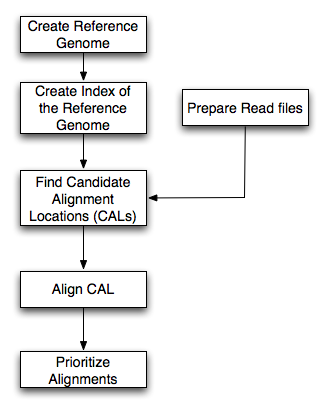
\includegraphics[scale=0.45]{figures/workflow.png} 

\caption{\small Overall workflow for a mapping procedure using BFAST.
  In this work, we focus on the step for finding Candidate Alignment
  Locations (CALs).}
  \label{fig:workflow-bfast} 
\end{figure}

\begin{table}
\begin{tabular}{|c|c|c|c|} 
  \hline BFAST & Description & Features for \\ command & & Parallelism
  \\ \hline \hline \texttt{fasta2brg} & creation of & multiple \\ &a ref. genome &
  independent \\ & & contigs \\ \hline
  \texttt{solid2fastq} & preparation of & multiple sequence \\ & short
  read files & read files\\ \hline

\texttt{bfast index} & creation  & multi-threading \& \\
& of reference  & low memory  \\ 
&genome indexes&option \\
 
  \hline
\texttt{bfast match} & finding Candidate   &  multi-threading \& \\

& Alignment &  parallel execution \\
& Locations (CALs) & \\\hline
\texttt{bfast localalign} & alignment of&   parallel execution \\
&  each CAL   & \\

  \hline
\texttt{bfast postprocess} & prioritization   &  parallel execution \\ 
& of alignments & \\
\hline


\hline
\end{tabular} \caption{Description of BFAST commands and features for parallel and multi-threading execution}
 \label{table:bfast-summary} 
\end{table}


\subsection{BFAST: Characteristics}

\begin{figure}
 \centering
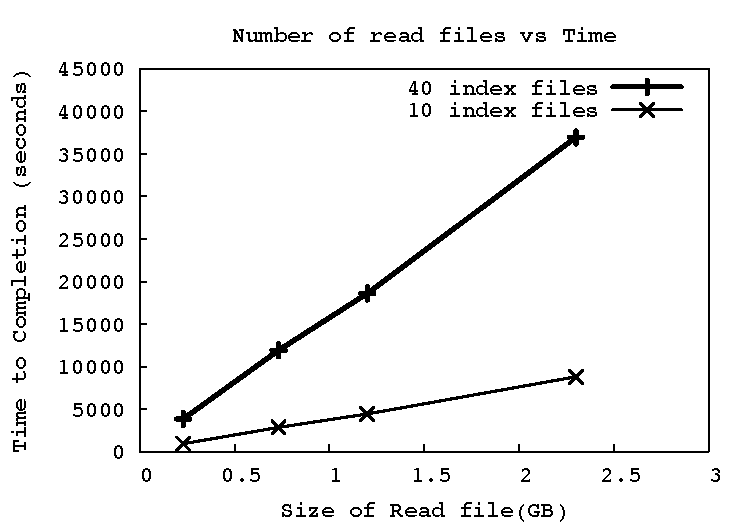
\includegraphics[scale=0.66]{figures/readsvstime.pdf}
%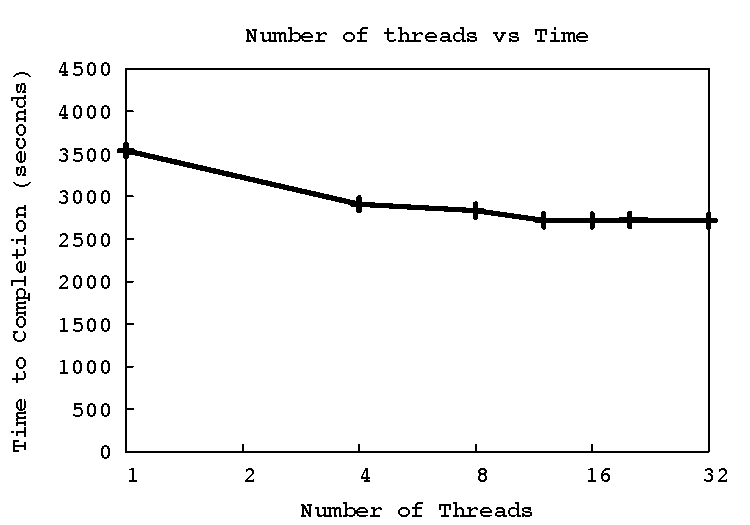
\includegraphics[scale=0.66]{figures/threadsvstime.pdf} 

\caption{\small The time-to-completion of the 'bfast match' step is
  measured by varying the size of short read file.  Two lines
  represent two cases differing in the low memory option, which
  results in the different number of index files.  Human genome (hg18)
  chromosome 21 is used as the reference genome. \jhanote{Need to say
    what the two lines in the left graph are, and what is the message
    we want to convey from showing the difference}}
  \label{fig:parallel-execution} 
 \end{figure}


\begin{table}
\begin{tabular}{|c|c|c|c|} 
  \hline 
   & Human (hg18) & Burkerholderia   \\ 
& & Glumae (BGR1)\\   
   
   \hline
 \underline{Reference Genome}   \\
    \# of base pairs (bp) &  3 Gbp & 7.3 Mbp \\
   Genome Structure &   23 chromosome  & 2 chromosomes  \\  
   &   pairs & \& 4 plasmids \\
    Volume of indexes  & approx. 12 GB  & approx. 447 MB  \\
      \hline
    \underline{ Short Reads}   \\
        \underline{ Sequence Data}   \\
  Type of  &  Exome  & Whole \\
  
Genome Analysis  &  &  Genome \\
&& Resequencing \\
  Sequencing Platform & ABI SOLiD  &  Illumina GA2 \\
  Sequencing   & 8.7 GB & 5.4 GB \\
  Data Volume&&\\
  
  
  \hline
  \underline{ BFAST mapping}  \\
  Minimal disk &  approx. 130 GB   &    approx. 10 GB   \\
total space required & &\\
\hline
\end{tabular} \caption{The information about the size of reference genomes, volumes of datasets from Next Generation Sequencing (NGS) platforms and disk space required during the mapping calculation with BFAST is summarized assuming all calculations are carried out with a single machine.}
 \label{table:two-genomes} 
\end{table}



\begin{table}
 \begin{tabular}{|c|c|c|c|} 
 \hline 
Read file & Index files & Appx. required disk space \\
 \hline
40 &  40 & 67 GB \\
20 & 40 & 70 GB \\
40 & 10 & 54 Gb \\ 

 \hline
 \end{tabular}
 \label{table:diskspace} 
 \caption{this table shows required disk space in different cases when all the read files are processed concurrently \jhanote{Sharath, please explain how the third column can be derived
  from the first two columns of the table}}
\end{table}



First, performance gains with multi-threading are marginal showing only 30 \% speed up when reaches the limit with all of the number of free cores being used.  Also, it is apparent that the option has a limitation only until the number of required thread becomes equal to the total available cores in a given system, 12 cores in the case of results in Fig.~\ref{fig:parallel-execution}.

The disk space required per each read file is constant given all the other size and read file size is the same. Because bfast matching creates several temperory files while its running. It include one temporary file for read file, ten temperory files for each index mask, some temporary files depending on the d option (d=0, 1 temp file, d=1 4 temprory files). ofcourse all these temp files are deleted after each bfast match run. The disk space required in concurrent run of several read files in Matching phase is important because if the amount of disk space required exceeds the available limit bfast fails. This plays a major role in distribution of computation depending upon the allowed disk space on each machine. 

\subsubsection{Computational Requirements}

An understanding of computational requirements for carrying out BFAST steps, in particular the "bfast match" step,is critically important for a infrastructure development in which a target genome-wde analysis tool is effectively provided to a scientific community as a scalable application,   The overall execution of BFAST, or any short read mapping tool, is dependent upon biological contexts such as a type of a target reference genome and a high-throughput sequencing technique generating short read sequences, data structure for parallel/concurrent execution, parallelism support such as multi-threading, and more importantly the utilization of such parameters with available computing architectures with respect to parallel execution capabilities and data management.  

In Table~\ref{table:two-genomes}, we summarize the information related to such parameters. For example, we investigated two genome datasets that are representative of biological diversity, an eucaryote system, human, and a microbe, Burkerholderia Glumae\cite{kim2011}.  Two genomes differ in the size and the genome structure of reference genomes, and types of sequencing protocols.  Importantly, the two different genomes display widely different data sizes in terms of the reference genome sequence, short reads data, and required disk space for carrying out the mapping with BFAST. 

As an investigation for computational requirements, first, we measure the time-to-completion for "bfast match" step while varying the size of a read file.  The results as shown in Fig.~\ref{fig:parallel-execution}, it is found that a linear scaling in time-to-completion vs. the size of read file is well satisfied, indicating the parallel option with multiple read files is a useful strategy of scaling out, i.e.  using more cores with a smaller size of read files.  Secondly, the low memory option that creates more index files require a longer calculation time as found with the comparison between 40 index files $(d = 1)$ vs. 10 index files ($ d = 0 $) ($n_m = 10$ is used).   


\jhanote{Joohyun: Please organize each description addressing each of
  the following points: (i) Brief outline of the scientific problem,
  (ii) What are the challenges, (iii) estimates of volumes of data
  involved, distributed or not?, number of tasks, are they coupled or
  uncoupled -- what is the level of coupling between tasks?}


 \begin{table}
 \begin{tabular}{|c|cc|} 
 \hline 
Distributed &  HPC Grid &  Cloud \\ 
Environment && (Eucalyptus)\\
\hline
 &  Louisiana Optical & FutureGrid \\
& Network Initiative  & \\
System  Name &  QB/Small Linux Clusters   &  INDIA/SIERRA \\
Disk Space  Limit  &  QB : unlimited  &    \\
                         &  Small Linux Clusters : 100 GB  &  \\
 \hline
 \end{tabular}
\caption{Specification of two distributed environments.  \jkimnote{need to fill Cloud systems}}
\label{table:two-systems} 
\end{table}
 
\subsubsection{Characterising Data Requirements}

\jhanote{Lines 86-87, In a nutshell: the operating data-set does not depend on the size/number of read files but does depend on the size/number of index files}

Mapping with BFAST should deal with the data for a reference genome, short reads, and processed data generated in each step.  Particularly, the temporary data generated during 'bfast match' step needs a careful attention due to their significant size and more importantly a characteristic aspect such that the size depends on how the step is executed, for example, concurrently vs. serially, or centralized storage vs. distributed storage, or the low memory option (i.e. the number of index files).
   
The overall information for data requirement is found with Table~\ref{table:two-genomes}, Table~\ref{table:diskspace} and Fig.~\ref{fig:diskspace}.   Generally, fragmentation of data sets is a primary idea to mitigate a storage requirement as well as computing time.  For example, as we mentioned above, separating short reads into multiple files is a good option with distributed computing resources.  While a reference genome index should be treated as a whole, there is a possible idea to break a reference genome.  For example, breaking a reference genome into many independent sets is possible, considering the fact that many organisms are composed of independent parts, for example, chromosomes and plasmids or that possible multiple contigs that represents discontinued genome sequences would exist as a reference genome.  Indeed, the human genome in Table~\ref{table:two-systems} with huge data volume as a whole is the case that combining ideas to split the target genome with all possible options ranging from biology to computing technologies is needed to overcome challenges arising from the data volume and computation.   


\begin{figure}
 \centering
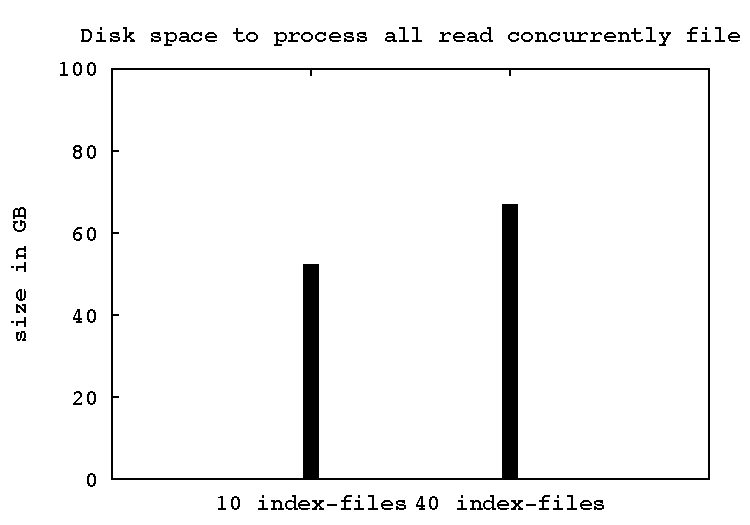
\includegraphics[scale=0.66]{figures/diskspace.pdf}
\caption{\small Disk space requirement for the cases that all read
  files are processed concurrently in a single storage (A and B) is
  compared to one for the cases when each single read file is
  processed alone (C and D).  Also, the cases with the low memory
  option producing 40 index files (A and C) are compared to the cases
  without the low memory option that produce 10 index files (B and
  D). \jhanote{Remove C and D ot later possibly}}
  \label{fig:diskspace} 
 \end{figure}






\section{Mapping using Distributed, Scalable Architectures}

\subsection{Existing Solutions: Limitations and Challenges}

\jhanote{Here we need to define what solutions are currently employed,
  what works well what doesn't}

Recently, cloud computing and environments for genome-wide analysis
and infrastructure development have drawn significant attention and
interesting outcomes were reported\cite{taylor2010,cloudburst,
  cloudblast, langmead2009, langmead2010,gatk, halligan2009}

\begin{itemize*}
\item GATK\cite{gatk}
\item CloudBurst\cite{cloudburst}
\item CouldBlast\cite{cloudblast}
\item SNP finding and RNA-seq with Cloud\cite{langmead2009, langmead2010}
\end{itemize*}

In spite of successful progress from such efforts, the primary
challenges that we want to resolve, and improve are as follow.
%\begin{enumerate}
\begin{itemize*}
\item Agility for heterogeneous computing architecture
\item Extensibility and quick development cycles for a new bioinformatics tool
\item Scalability with a non-intrusive execution of a target tool  
%\end{enumerate}
\end{itemize*}


\subsection{Understanding BFAST on a Local (Single) Resource}

\subsubsection{$T_{C}$ on $N_t$ and $N_c$}

 \begin{figure}
 \centering
%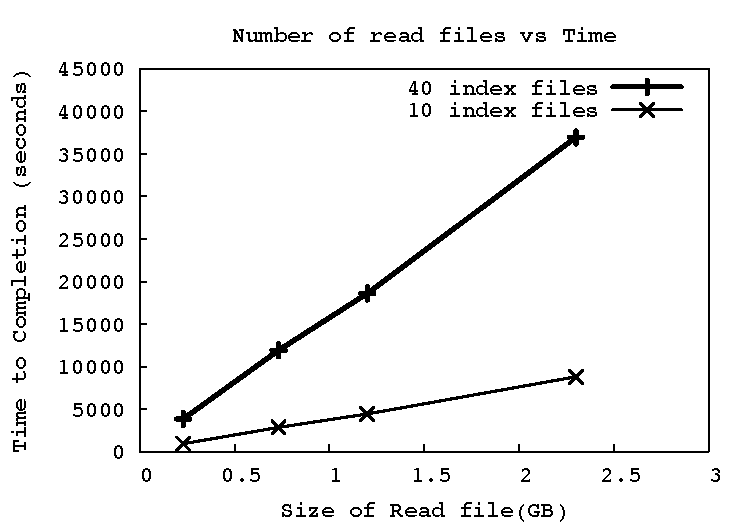
\includegraphics[scale=0.66]{figures/readsvstime.pdf}
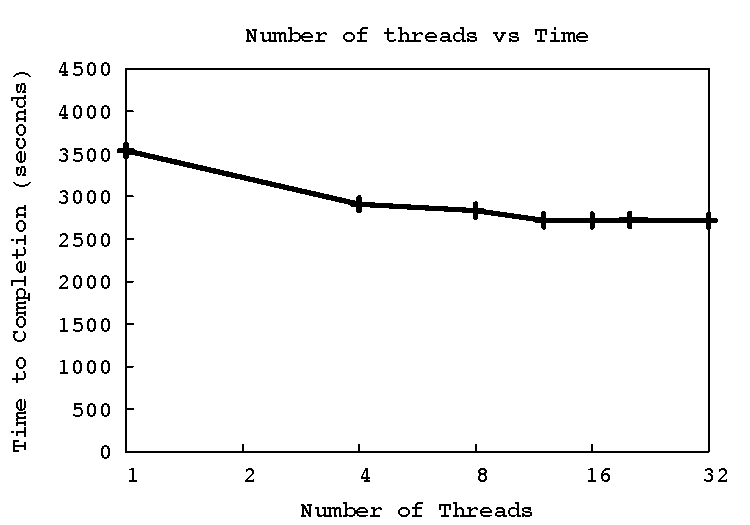
\includegraphics[scale=0.66]{figures/threadsvstime.pdf} 

\caption{\small The multi-threading capability measurement.  The 'bfast match' 'step is measured by varying the number of cores for multi-threading execution.  The node tested has 12 cores.  Human genome (hg18) chromosome 21 is used as the reference genome. \jhanote{Need to say what the two lines in the left graph are, and what is the message we want to convey from showing the difference} \jhanote{I think we should use gnuplot for production quality graphs. Sorry -- but the quality makes a significant difference and Excel just does not cut it.}}
  \label{fig:parallel-execution} 
 \end{figure}
To determine how the bfast match performance changes with the different number of threads and processor we vary the number of threads for bfast job on a single machine with multiple cores. The results show that the performance was better when the number of cores is equal to number of threads which was also recommended setting in the Bfast manual. Further, when we increase number of threads more than available performance does not change much. When less number of threads are used than the available cores the performance decreases but marginal around half of the cores and significant with just single thread.


So even with multi-threading option provided by bfast, the performance
could be improved by using multiple cores/threads on the same node but
it gives us only marginal overall performance gain when processing all
the read files sequentially.

... \jhanote{needs merging} The results from our investigation are presented in
Fig.~\ref{fig:parallel-execution}. First, performance gains with
multi-threading are marginal showing only 30 \% speed up when reaches
the limit with all of the number of free cores being used.  Secondly,
the multiple read file option is useful as a strategy for scaling out,
i.e. with more cores operating correspondingly a smaller read file.
Thirdly, the low memory option that creates more index files require
longer calculation time as the comparison between 40 index files $(d =
1)$ vs. 10 index files ($ d = 0 $) and $n_m = 10$.


... \jhanote{needs merging} Computational requirements vary also with
how to configure parallel/multi-threading execution patterns.  Since
BFAST provides its intrinsic support for multi-threading and parallel
execution, we examined computational requirements while varying
configurations for such parallel strategies.  For example, according
to the results shown in Fig.~\ref{fig:parallel-execution}, it is
obvious that dividing a large volume of short reads data into many
independent runs is a good strategy while multi-threading support is
limited by available cores in a same node.  Also the results in
Fig.~\ref{fig:parallel-execution} find that the low memory option that




\subsubsection{Understanding I/O}
{
To understand the how I/O of the system influences the performance of bfast matching four different experiments were conducted keeping the amount of data processed constant and number of threads used also as constant but for the first three. In the first experiment we just perform one bfast match for a large read file of size with four threads and four cores. In the second experiment two bfast matches concurrently with almost half the size of read file but half of the threads used in the first one.Similarly, in the third experiment we run four bfast matches concurrently with almost quarter the size read file used but the in the first experiment and one thread each. Fourth one is similar to third except in the number of threads 4 threads per bfast job is used but using just 4 cores.

 \begin{table}
 \begin{tabular}{|c|c|c|c|} 
 \hline 
Read File Size & Threads  & BFAST Tasks & Time to \\
& per Read File&  &  Completion \\  \hline
2.3 GB &  4 & 1 & 36942 s \\
1.2 GB & 2 & 2 & 19618 s \\
0.732 GB & 1 & 4 & 28299 s\\ 
0.732  GB & 4 & 4 & 25215 s\\

 \hline
 \end{tabular}
 \label{table:understand I/o} 
 \caption{Computing time for the 'bfast match' step with a single node.  Under the restriction such that the tested node has 4 cores, the time-to-completions are compared with varying conditions regarding the size of read files, the number of thread for each 'bfast match', and number of the 'bfast match' executed concurrently.}
\end{table}

These experiments show that use of 2 threads per bfast matches simultaneously on a four core node is the optimal configuration for time to completion. Because it balances each thread per core but  running the two bfast jobs per node at the same time. Thus shows advantage of running multiple bfast matches simultaneously. 


}

\jhanote{Lines 44-47 of the Excel Sheet here}

\subsection{Distributed Adaptive Runtime Environment}

To execute a scientific application using heterogeneous distributed
computing resources, we develop the Distributed Adaptive Runtime
Environment (DARE) framework\cite{dareurl}.  The framework is compose
of an open source Web application framework, Pylons and middleware of
the application management system built upon SAGA an BigJob
abstraction\cite{saga-ccgrid10,saga-royalsoc,saga-web,jha2009developing,ecmls10}.
This combination of the open source technology and the application
management system enables us to develop a lightweight, extensible,
full-fledged distributed computing science gateway quickly and
effectively\cite{pylonsurl}.

Considering a daunting size of data, in particular large genomes such as human as summarized in Table~\ref{table:two-genomes} and corresponding long computing times when carried out with a single or moderate size of clusters, parallel/concurrent execution of the target analysis with BFAST are desirable.  First, biological information could be utilized for such parallel execution. For example, the short read sequences in fastq format could be split into many files that are needed separately for parallel mapping.  At the last stage, all mapped results could be combined with available tools such as SAMTools\cite{samtools}.   Additionally, a reference genome could be divided into many if each dataset contains independent contigs.  For example, each chromosomes or plasmids in microbes could be a separated sub-genome sequence contig.  However, note that indexes of an entire contig should be used together, regardless of the low memory option that allows to store indexes in many files, which is in fact the major obstacle to require a large disk space.

We implement the above data fragmentation scheme on grids and clouds with the same runtime environment using SAGA/BigJob\cite{saga-royalsoc,saga-ccgrid10, ecmls10}.  In our implementation, all the parallel tasks of BFAST steps are defined as SubJobs in BigJobs.  It is possible to assign many cores for each SubJob with the configuration of BigJob before submitting BigJobs. 
  
...\jhanote{needs merging} Most importantly, while the implementation
of multiple parallel tasks indicates advantages of distributed
multiple resource utilization, the large volume and variation of data
sizes associated with genome sequence data as well as minimally
required disk space needs to pay attention since in some cases, data
size itself prohibits to carry out the analysis in a computing
resource that lacks the demanded requirements, indicating the
significance of agile runtime environment that drives a dynamical
configuration and utilization of distributed resources.

\subsection{Execution on Grids and Clouds}

\subsubsection{Using BFAST On Distributed HPC Resources}

Following is the implementation described above, the execution of
mapping calculations using BFAST was tested with our runtime
environment built with the DARE framework.  Results were obtained with
a HPC grid and a Cloud environment, which demonstrate the capability
of our runtime environment for the mapping tool on distributed
heterogeneous computing resources. \jhanote{Before we say what we are
  presenting, please present a ``why and how'', i.e., outline the
  experiments}

First of all, in Table~\ref{table:bigjob-loni}, we presented the
measured time-to-completion for the step 'bfast match' with different
configurations that include the variation of the number of threading
used for each task and the number of cores (and also the number of
nodes).  These results clearly show i) effective job submission and
sub task management trough BigJob in spite of a large number of
subtasks up to 40 ii) requirement of sufficient number of cores
through available distributed computing resources (see I and II
compared to III and IV that requires many rounds of parallel
executions due to limited number of cores) that completes parallelism
with multiple read files.  In particularly, the observation with (ii),
along with the observation already shown in
Fig.~\ref{fig:parallel-execution} that observed a marginal performance
gain with the option for increasing number of threading, is clearly
supported by the results shown in Fig.~\ref{} once again that shows
the result in that without sufficient cores available from distributed
resources and dynamically adapted task distribution, achieving the
efficient execution of a target calculation is challenging.

\begin{table}
 \begin{tabular}{|c|cc|} 
 \hline 
Distributed &  HPC Grid &  Cloud \\ 
Environment && (Eucalyptus)\\
\hline
 &  Louisiana Optical & FutureGrid \\
& Network Initiative  & \\
System  Name &  QB/Eric   &  INDIA/SIERRA \\
 \hline
 \end{tabular}
\caption{Specification of two distributed environments}
\label{table:two-systems} 
\end{table}


 \begin{table}
 \begin{tabular}{|ccccc|c |} 
 \hline 
ID & BigJob Size  &  Tasks & Size of  & Threads per  &  Computing  \\
   & Cores(Nodes) &  & Read File & each Task &  Time\\\hline
I   & 80(8) &  40 & 0.209 GB & 2 & 1h 6 m 6 s \\
II  & 40(8)  &  20 & 0.435 GB & 2 & 2 h 13 m 51 s\\
III & 12(4)  & 40  & 0.209 GB & 2 & 7 h 10 m 7 s \\
IV & 12(4)  & 20 & 0.435 GB & 2 &  6 h 37 m 52  \\
\hline
\end{tabular}
\caption{Performance comparison among parallel implementation using
  SAGA/BigJob with a HPC grid, LONI. One BigJob is submitted with the
  number of SubJobs indicated in the column for the number of tasks
  which is equivalent to the number of read files. \jhanote{This table
    needs to be fixed -- crosses the page. Are Case I/II/III/IV the
    same as A/B/C/D? } }
  \label{table:bigjob-loni} 
\end{table}


\subsubsection{Using BFAST on Clouds and Grids}

... \jhanote{needs merging} In the Grid implementation first all the
data required in the steps was transferred to machine's work directory
where we want to start the BigJob. The BFAST was installed in the home
directory and the executables path for job description of subjobs was
given accordingly.

... \jhanote{needs merging} In the cloud implementation all the data
required was transferred into the walrus because of the data size
limitation of the storage space in the running VM. Multiple VM's can
be started at once and the data in the walrus is mounted onto all the
running VM while booting the Virtual Machine. Thus all the VM can have
access to data and can process concurrently


To determine whether to use large number of small VM's or to use few
big VM's. with help of bigjob cloud implementation we designed two
experiments. In the first experiment four VM's with 2 cores each were
started and four bfast matches with one bfast on each one using SAGA
bigjob . In the second experiment a large VM with 8 cores is started
and 4 bfast jobs were launched on the same VM simultaneously using
SAGA bigjob.

 \begin{table}
 \begin{tabular}{|c|c|c|} 
 \hline 
VM's & VM type and Cores  & Time to  \\ 
&per VM& completion\\ 
\hline
4 &  2 & 1080 s \\
1 & 8 & 1020 s \\
 \hline 
 \end{tabular}
 \label{table:cloud-VM} 
 \caption{The time-to-completion is compared between the case of multiple VMs and the case of single VM}
\end{table}

Thus when same workload is distributed across multiple VM's has a
marginal gain over the one single large VM.

\jhanote{Need to refer to Table\ref{table:cloud-VM}}


\section{Concluding Remarks}
We present our analyses with two genome systems representing a
eukaryote and a prokaryote, respectively, using a HPC grid and a Cloud
environment for an understanding of conditions of a scalable
cyberinfrastructure for an effective execution of mapping, and
consequently genome-wide analyses.  Based on our results, we conclude
that an infrastructure to run with a proper configuration for
concurrent tasks benefits genome-wide analysis and such a
configuration is optimized only when parameters from biological
contexts as well as limitations and potentials of distributed
computational resources are taken into account together.  For that
purpose, our DARE framework provides an efficient solution.



\bibliographystyle{abbrv}
\bibliography{ecmls11}


\end{document}


